% Options for packages loaded elsewhere
\PassOptionsToPackage{unicode}{hyperref}
\PassOptionsToPackage{hyphens}{url}
\PassOptionsToPackage{dvipsnames,svgnames,x11names}{xcolor}
%
\documentclass[
]{agujournal2019}

\usepackage{amsmath,amssymb}
\usepackage{iftex}
\ifPDFTeX
  \usepackage[T1]{fontenc}
  \usepackage[utf8]{inputenc}
  \usepackage{textcomp} % provide euro and other symbols
\else % if luatex or xetex
  \usepackage{unicode-math}
  \defaultfontfeatures{Scale=MatchLowercase}
  \defaultfontfeatures[\rmfamily]{Ligatures=TeX,Scale=1}
\fi
\usepackage{lmodern}
\ifPDFTeX\else  
    % xetex/luatex font selection
\fi
% Use upquote if available, for straight quotes in verbatim environments
\IfFileExists{upquote.sty}{\usepackage{upquote}}{}
\IfFileExists{microtype.sty}{% use microtype if available
  \usepackage[]{microtype}
  \UseMicrotypeSet[protrusion]{basicmath} % disable protrusion for tt fonts
}{}
\makeatletter
\@ifundefined{KOMAClassName}{% if non-KOMA class
  \IfFileExists{parskip.sty}{%
    \usepackage{parskip}
  }{% else
    \setlength{\parindent}{0pt}
    \setlength{\parskip}{6pt plus 2pt minus 1pt}}
}{% if KOMA class
  \KOMAoptions{parskip=half}}
\makeatother
\usepackage{xcolor}
\setlength{\emergencystretch}{3em} % prevent overfull lines
\setcounter{secnumdepth}{5}
% Make \paragraph and \subparagraph free-standing
\ifx\paragraph\undefined\else
  \let\oldparagraph\paragraph
  \renewcommand{\paragraph}[1]{\oldparagraph{#1}\mbox{}}
\fi
\ifx\subparagraph\undefined\else
  \let\oldsubparagraph\subparagraph
  \renewcommand{\subparagraph}[1]{\oldsubparagraph{#1}\mbox{}}
\fi


\providecommand{\tightlist}{%
  \setlength{\itemsep}{0pt}\setlength{\parskip}{0pt}}\usepackage{longtable,booktabs,array}
\usepackage{calc} % for calculating minipage widths
% Correct order of tables after \paragraph or \subparagraph
\usepackage{etoolbox}
\makeatletter
\patchcmd\longtable{\par}{\if@noskipsec\mbox{}\fi\par}{}{}
\makeatother
% Allow footnotes in longtable head/foot
\IfFileExists{footnotehyper.sty}{\usepackage{footnotehyper}}{\usepackage{footnote}}
\makesavenoteenv{longtable}
\usepackage{graphicx}
\makeatletter
\def\maxwidth{\ifdim\Gin@nat@width>\linewidth\linewidth\else\Gin@nat@width\fi}
\def\maxheight{\ifdim\Gin@nat@height>\textheight\textheight\else\Gin@nat@height\fi}
\makeatother
% Scale images if necessary, so that they will not overflow the page
% margins by default, and it is still possible to overwrite the defaults
% using explicit options in \includegraphics[width, height, ...]{}
\setkeys{Gin}{width=\maxwidth,height=\maxheight,keepaspectratio}
% Set default figure placement to htbp
\makeatletter
\def\fps@figure{htbp}
\makeatother
\newlength{\cslhangindent}
\setlength{\cslhangindent}{1.5em}
\newlength{\csllabelwidth}
\setlength{\csllabelwidth}{3em}
\newlength{\cslentryspacingunit} % times entry-spacing
\setlength{\cslentryspacingunit}{\parskip}
\newenvironment{CSLReferences}[2] % #1 hanging-ident, #2 entry spacing
 {% don't indent paragraphs
  \setlength{\parindent}{0pt}
  % turn on hanging indent if param 1 is 1
  \ifodd #1
  \let\oldpar\par
  \def\par{\hangindent=\cslhangindent\oldpar}
  \fi
  % set entry spacing
  \setlength{\parskip}{#2\cslentryspacingunit}
 }%
 {}
\usepackage{calc}
\newcommand{\CSLBlock}[1]{#1\hfill\break}
\newcommand{\CSLLeftMargin}[1]{\parbox[t]{\csllabelwidth}{#1}}
\newcommand{\CSLRightInline}[1]{\parbox[t]{\linewidth - \csllabelwidth}{#1}\break}
\newcommand{\CSLIndent}[1]{\hspace{\cslhangindent}#1}

\usepackage{url} %this package should fix any errors with URLs in refs.
\usepackage{lineno}
\usepackage[inline]{trackchanges} %for better track changes. finalnew option will compile document with changes incorporated.
\usepackage{soul}
\linenumbers
\makeatletter
\makeatother
\makeatletter
\makeatother
\makeatletter
\@ifpackageloaded{caption}{}{\usepackage{caption}}
\AtBeginDocument{%
\ifdefined\contentsname
  \renewcommand*\contentsname{Table of contents}
\else
  \newcommand\contentsname{Table of contents}
\fi
\ifdefined\listfigurename
  \renewcommand*\listfigurename{List of Figures}
\else
  \newcommand\listfigurename{List of Figures}
\fi
\ifdefined\listtablename
  \renewcommand*\listtablename{List of Tables}
\else
  \newcommand\listtablename{List of Tables}
\fi
\ifdefined\figurename
  \renewcommand*\figurename{Figure}
\else
  \newcommand\figurename{Figure}
\fi
\ifdefined\tablename
  \renewcommand*\tablename{Table}
\else
  \newcommand\tablename{Table}
\fi
}
\@ifpackageloaded{float}{}{\usepackage{float}}
\floatstyle{ruled}
\@ifundefined{c@chapter}{\newfloat{codelisting}{h}{lop}}{\newfloat{codelisting}{h}{lop}[chapter]}
\floatname{codelisting}{Listing}
\newcommand*\listoflistings{\listof{codelisting}{List of Listings}}
\makeatother
\makeatletter
\@ifpackageloaded{caption}{}{\usepackage{caption}}
\@ifpackageloaded{subcaption}{}{\usepackage{subcaption}}
\makeatother
\makeatletter
\@ifpackageloaded{tcolorbox}{}{\usepackage[skins,breakable]{tcolorbox}}
\makeatother
\makeatletter
\@ifundefined{shadecolor}{\definecolor{shadecolor}{rgb}{.97, .97, .97}}
\makeatother
\makeatletter
\makeatother
\makeatletter
\ifdefined\Shaded\renewenvironment{Shaded}{\begin{tcolorbox}[frame hidden, boxrule=0pt, sharp corners, interior hidden, enhanced, breakable, borderline west={3pt}{0pt}{shadecolor}]}{\end{tcolorbox}}\fi
\makeatother
\makeatletter
\makeatother
\ifLuaTeX
  \usepackage{selnolig}  % disable illegal ligatures
\fi
\IfFileExists{bookmark.sty}{\usepackage{bookmark}}{\usepackage{hyperref}}
\IfFileExists{xurl.sty}{\usepackage{xurl}}{} % add URL line breaks if available
\urlstyle{same} % disable monospaced font for URLs
\hypersetup{
  pdftitle={Fish species size distributions in a changing climate},
  pdfauthor={Freddie J. Heather; Shane Richards; Asta Audzijonyte},
  pdfkeywords={Fish body size, Temperature size rule, Empirical size
distribution, Body size distribution},
  colorlinks=true,
  linkcolor={blue},
  filecolor={Maroon},
  citecolor={Blue},
  urlcolor={Blue},
  pdfcreator={LaTeX via pandoc}}

\journalname{Nature}

\draftfalse

\begin{document}
\title{Fish species size distributions in a changing climate}

\authors{Freddie J. Heather\affil{1}, Shane Richards\affil{2}, Asta
Audzijonyte\affil{1}}
\affiliation{1}{Institute for Marine and Antarctic Studies, University
of Tasmania, }\affiliation{2}{School of Natural Sciences, University of
Tasmania, }
\correspondingauthor{Freddie J. Heather}{freddie.heather@utas.edu.au}


\begin{abstract}
Abstract goes here
\end{abstract}



\hypertarget{sec-background}{%
\section{Background}\label{sec-background}}

Body size is a key trait in determining how organisms interact with
their environment, this is particularly true for marine organisms, where
body size is a strong predictor of trophic position\textsuperscript{1},
growth rate, and predation mortality\textsuperscript{2}. Giometto et
al.\textsuperscript{3}, using the spherical diameter of unicellular
protists, identified that the mean body size of a species, was
sufficient to describe the entire body size distribution. The authors
conjectured that this may hold for multicellular organisms. Here, we
test this conjecture using 15 millon+ inidividuals from 1064 fish
species.

\hypertarget{sec-results-discussion}{%
\section{Results \& discussion}\label{sec-results-discussion}}

We found that the variance parameter of the lognormal distribution was
constant across the fitted mean parameter of the lognormal distribution
(Figure~\ref{fig-param-regression} A), further we found a consistent
relationship between the standard deviation and the mean of the normal
distribution fitted to observed body size
(Figure~\ref{fig-param-regression} B). This is to say the mean size of
the species is sufficient to describe the overall body size
distribution. For both data sources, continuous and binned, we found the
patterns between the mean and variance parameters of the lognormal
distribution held, with sdlog = 0.39 \(\pm\) 0.007 (Reef Life Survey,
binned data) and 0.3 \(\pm\) 0.03 (Cryptobenthic fish, continuous). For
normal distribution, we found a consistent relationship

\begin{figure}

{\centering 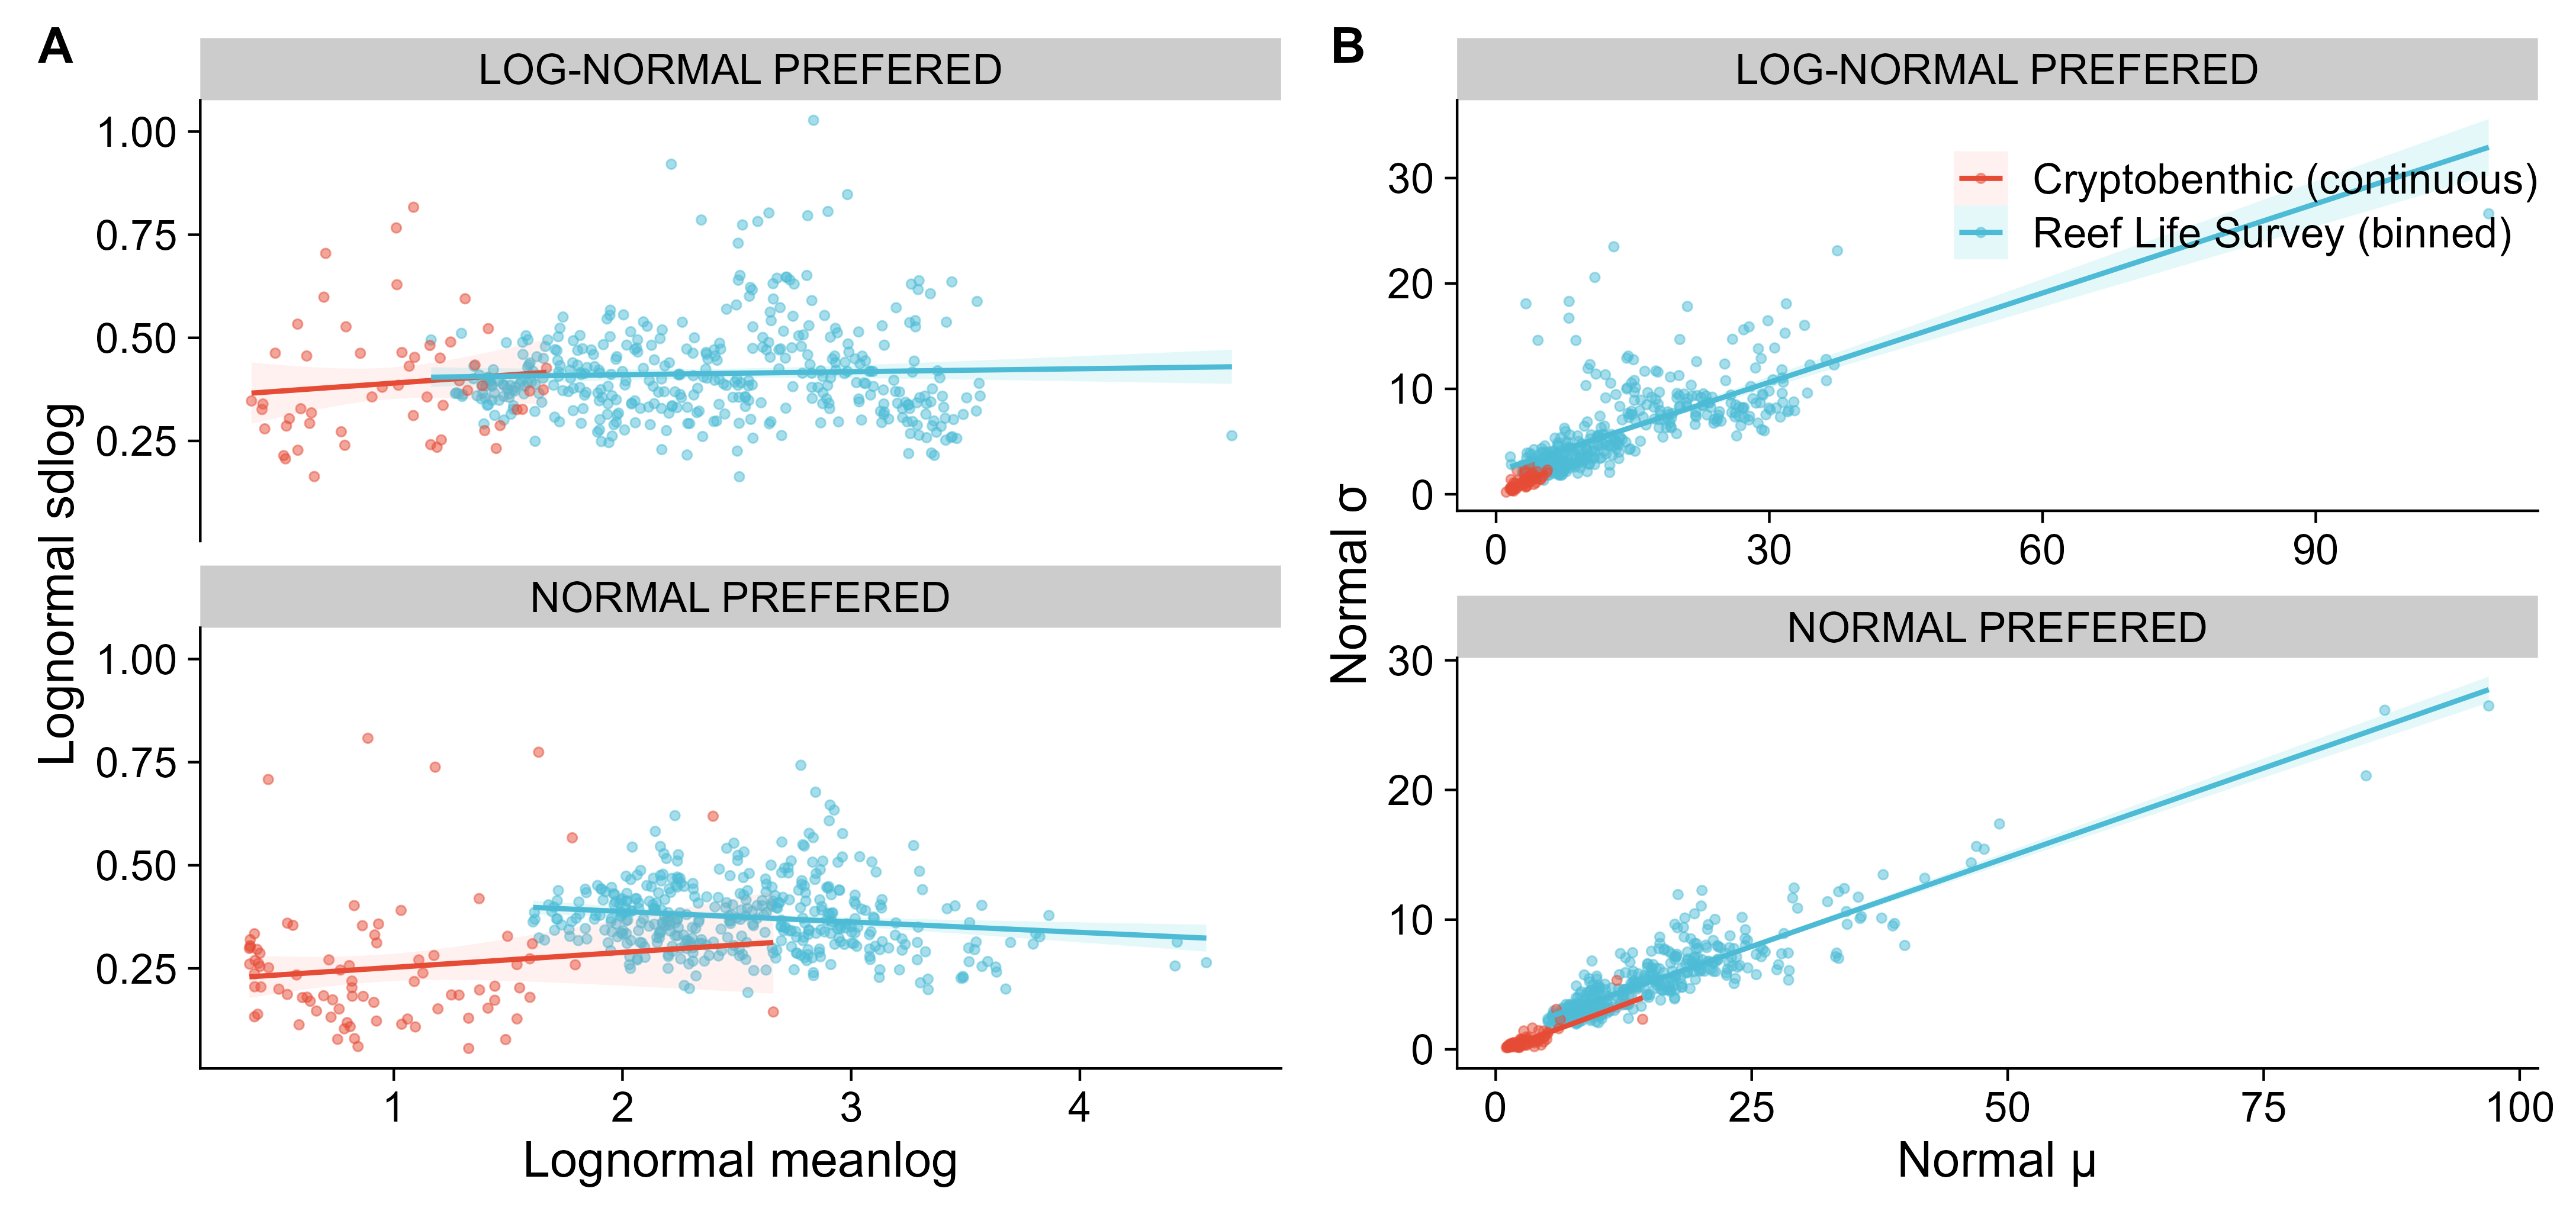
\includegraphics{ms_figures/param_regression.png}

}

\caption{\label{fig-param-regression}Mean size is sufficient to describe
overall body size distribution.}

\end{figure}

\hypertarget{sec-methods}{%
\section{Methods}\label{sec-methods}}

\hypertarget{body-size-data-sources}{%
\subsection{Body size data sources}\label{body-size-data-sources}}

Fish body size data were obtained through two sources: Reef Life Survey
(RLS; 15M+ individuals, binned body size)\textsuperscript{4}, and
Cryptobenthic reef fish (CBF; 8K+ individuals, continuous body
size)\textsuperscript{5}.

RLS surveys involve an underwater visual census method along 50m
transect line, with a diver searching 5m either side of the transect
line, the body size of the fish is estimated to the nearest body size
bin (2.5, 5, 7.5, 10, 15, 20, 25, 30, \ldots, 400cm).

The second data source was from field collections using enclosed
clove-oil stations at six reefs; Moorea, GoO, AG, Lizard Island, Panama,
and Belize. Reef outcrops are selected, measured, and covered with a
bell-shaped fine mesh and tarpaulin, before being sprayed with a
clove-oil:ethanol solution (1:5). Fish are collected with tweezers and
placed in ziplock bags. See Brandl et al.\textsuperscript{5} for full
methods.

\hypertarget{data-filtering}{%
\subsection{Data filtering}\label{data-filtering}}

For binned body size data, we excluded body size distributions that
spanned fewer than four body size bins, we did not apply an exclusion
for the continuous data based on the range of body sizes. For binned
data we set a minimum count of 10 individuals per population to fit a
distribution, for the binned data, this minimum count was 100. We
performed a sensitivity analysis to these filtering parameters to show
that across a range of filters for minimum count, the overall result did
not substantially change.

\hypertarget{statistical-analysis}{%
\subsection{Statistical analysis}\label{statistical-analysis}}

All statistical analyses were performed using the statistical
programming language R\textsuperscript{6}, and in combination with the
statistical modelling language Stan\textsuperscript{7} for Bayesian
analyses.

Cryptobenthic fish body size data, on a continuous scale, were fitted to
one of two probability distributions, lognormal and normal, and to two
spatial scales; 1) the species-level and the localised (reef) scale.

\[
S \sim \mathcal{N}(\mu, \sigma)\\
S \sim \mathcal{LN}(\nu, \tau)
\]

Where S is the observed body size, N represents the lognormal
distribution and its parameters, and LN represents the lognormal
distribution here, we have used \(\nu\) and \(\tau\) as the location and
scale parameters of the lognormal distribution to avoid confusion with
\(\mu\) and \(\sigma\).

Reef Life Survey body size data, in body size bins, were also fit using
Stan, but using a method to account for the body size binning approach.
The probability of being within each RLS body size bin (e.g.~2.5cm) was
calculated as the integral the probability distribution between the
upper and lower bounds of the size bin (e.g.~between 3.75 and 1.25cm).
This probability was then normalised to the total detectability of the
RLS method (i.e.~Pr \textgreater1.25cm) under the assumption that
individuals less than 1.25cm would not be counted in the RLS approach.
This method was run for both the normal and lognormal distributions. The
likelihood of the model was defined as the summation of the probability
of the data given the model parameters. To account for misclassification
error in the binning of body size an additional small parameter
(\(\epsilon\)) was added that adjusts the bin probability by a small
amount, which also has the benefit of avoiding zero probability
estimates.

\[
Pr(B_b,K_k) = \int_{B_{il}}^{B_{iu}}\mathcal{N}(\mu_k, \sigma_k)\cdot C
\]

where, the normalising constant (c) is defined by the probability of
being less than 1.25cm;

\[
C = \int_{0}^{1.25}\mathcal{N}(\mu_k, \sigma_k)
\]

\hypertarget{conclusion}{%
\section{Conclusion}\label{conclusion}}

\hypertarget{refs}{}
\begin{CSLReferences}{0}{0}
\vspace{1em}

\leavevmode\vadjust pre{\hypertarget{ref-jennings_weak_2001}{}}%
\CSLLeftMargin{1. }%
\CSLRightInline{Jennings, S., Pinnegar, J. K., Polunin, N. V. \& Boon,
T. W. \href{https://www.jstor.org/stable/2693497}{Weak cross-species
relationships between body size and trophic level belie powerful
size-based trophic structuring in fish communities}. \emph{Journal of
Animal Ecology} 934--944 (2001).}

\leavevmode\vadjust pre{\hypertarget{ref-goatley_body_2016}{}}%
\CSLLeftMargin{2. }%
\CSLRightInline{Goatley, C. H. R. \& Bellwood, D. R.
\href{https://doi.org/10.1098/rspb.2016.1858}{Body size and mortality
rates in coral reef fishes: A three-phase relationship}.
\emph{Proceedings of the Royal Society B: Biological Sciences}
\textbf{283}, 20161858 (2016).}

\leavevmode\vadjust pre{\hypertarget{ref-giometto_scaling_2013}{}}%
\CSLLeftMargin{3. }%
\CSLRightInline{Giometto, A., Altermatt, F., Carrara, F., Maritan, A. \&
Rinaldo, A. \href{https://doi.org/10.1073/pnas.1301552110}{Scaling body
size fluctuations}. \emph{Proceedings of the National Academy of
Sciences} \textbf{110}, 4646--4650 (2013).}

\leavevmode\vadjust pre{\hypertarget{ref-edgar_systematic_2014}{}}%
\CSLLeftMargin{4. }%
\CSLRightInline{Edgar, G. J. \& Stuart-Smith, R. D.
\href{https://doi.org/10.1038/sdata.2014.7}{Systematic global assessment
of reef fish communities by the {Reef} {Life} {Survey} program}.
\emph{Scientific Data} \textbf{1}, 140007 (2014).}

\leavevmode\vadjust pre{\hypertarget{ref-brandl_demographic_2019}{}}%
\CSLLeftMargin{5. }%
\CSLRightInline{Brandl, S. J. \emph{et al.}
\href{https://doi.org/10.1126/science.aav3384}{Demographic dynamics of
the smallest marine vertebrates fuel coral reef ecosystem functioning}.
\emph{Science} \textbf{364}, 1189--1192 (2019).}

\leavevmode\vadjust pre{\hypertarget{ref-rcoreteam2022}{}}%
\CSLLeftMargin{6. }%
\CSLRightInline{R Core Team. \emph{\href{https://www.R-project.org/}{R:
A language and environment for statistical computing}}. (R Foundation
for Statistical Computing, 2022).}

\leavevmode\vadjust pre{\hypertarget{ref-standevelopmentteam2023}{}}%
\CSLLeftMargin{7. }%
\CSLRightInline{Stan Development Team.
\emph{\href{https://mc-stan.org}{Stan modeling language users guide and
reference manual, v2.21.0}}. (2023).}

\end{CSLReferences}

\begin{figure}[H]

{\centering 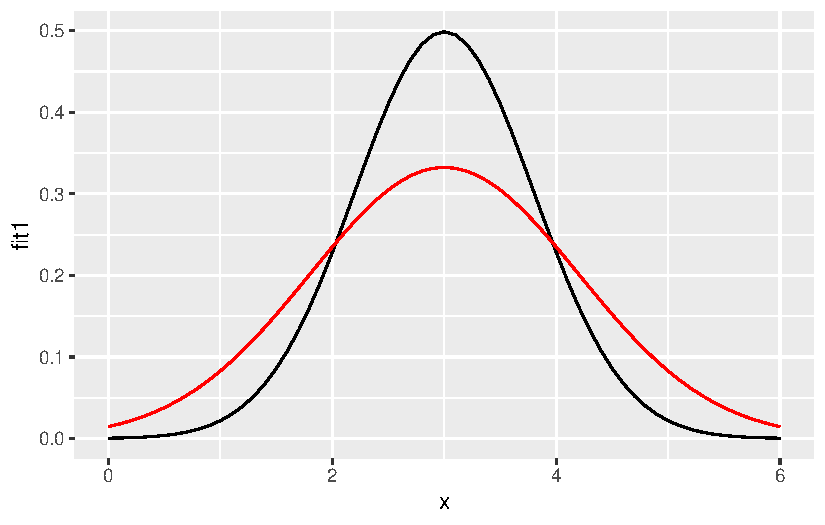
\includegraphics{index_files/figure-pdf/unnamed-chunk-2-1.pdf}

}

\end{figure}



\end{document}
